\chapter{Background}

\section{Embedded Databases}
\subsection{DuckDB}

\subsection{SQLite}

\section{Incremental View Maintenance}

\begin{tcbraster}[raster columns=2,raster equal height]
    \begin{definitionbox}{Views}
        \centerline{\textbf{Recompute on Access}}
        \begin{minted}{SQL}
CREATE VIEW my_view AS SELECT * FROM ..;            
        \end{minted}
        An alias for a query, typically a \mintinline{SQL}{SELECT} statement, that can be queried like a table. The view's query is used each time it is accessed.\cite{Postgres16Docs}
    \end{definitionbox}
    \begin{definitionbox}{Materialized Views}
        \centerline{\textbf{Recompute on Change}}
        Views with results cached. The contained query is only recomputed after a change in the data the query relies on. Beneficial for expensive queries that are frequently accessed and depend on infrequently changing data.
    \end{definitionbox}
\end{tcbraster}
\noindent
The aim of incremental view maintenance is to support views on data that \textbf{Never Recompute} in their entirety, but instead can updated \textit{incrementally} using changes applied to source relations.
\\
% diagram
\subsection{DBToaster}
DBToaster is an incremental view maintenance code generation tool, that generates C++, Spark (including a distributed spark target) and OCaml implementations from queries written in a subset of SQL.
\begin{center}
    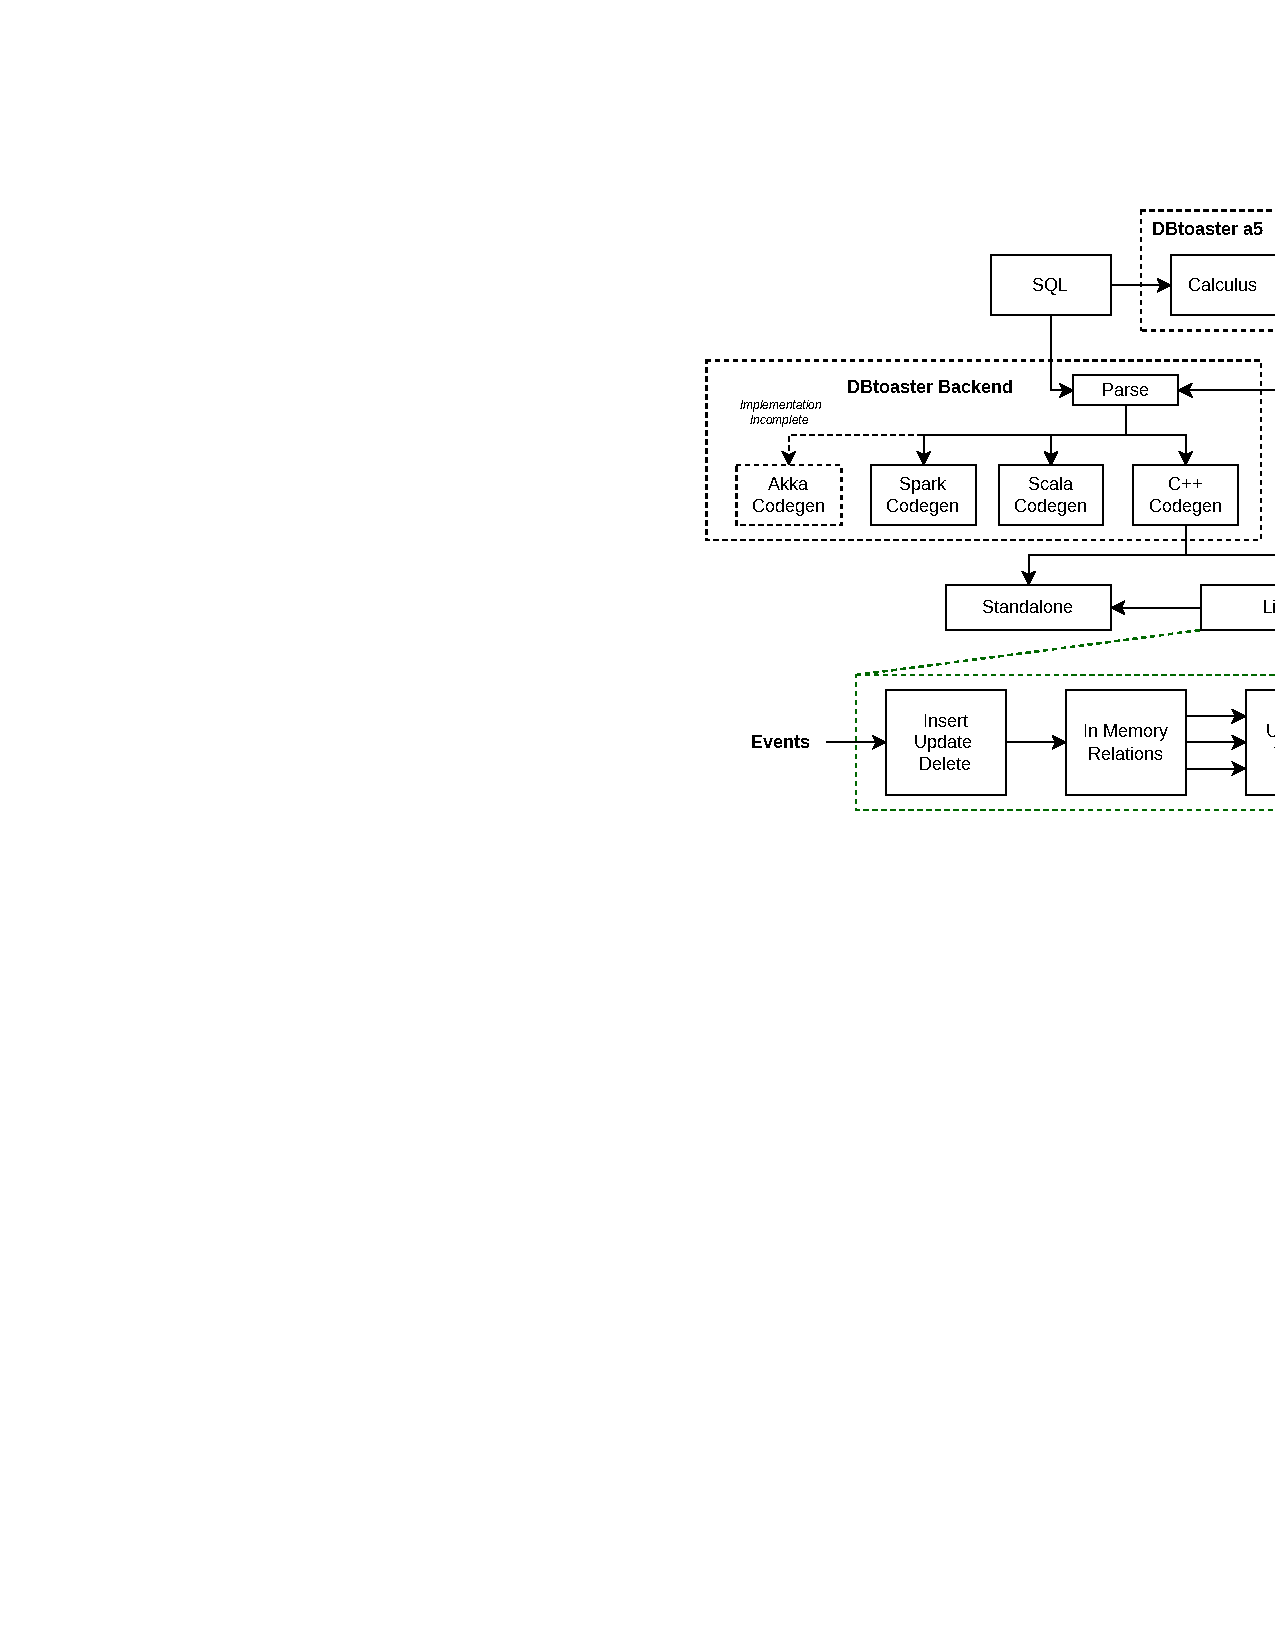
\includegraphics[width=\textwidth]{_drawio/background/images/dbtoaster_system.pdf}
\end{center}
\begin{center}
    \begin{tabular}{l p{.8\textwidth}}
        \textbf{SQL} & {
                A subset of SQL is supported to construct select queries on streams\cite{DBToasterSQLReference} of tuple changes.
                Tables are supported, but are static and cannot be modified after load.
            }
        \\
    \end{tabular}
\end{center}
\subsubsection{Incremental Calculus}
\subsubsection{Evaluation}

\subsection{Naiad/Materialize/Differential Dataflow}
\subsubsection{Evaluation}

\section{Domain Specific Languages}
\subsection{Language Integrated Queries}
\subsubsection{LINQ}

\subsubsection{sqlx}

\subsection{Rust Procedural Macros}

